\subsection{主纤维丛}

定义 1. --- 设 G 为拓扑群，B 为拓扑空间。以 B 为基、以 G 为群的（右）主纤维丛是指赋以 G 在 E 上的右作用 (A, I, p. 50) 且满足下列性质的 B-空间 (E, p)：

(FP) 对每一点 \(b\) （\(B\) 的），存在邻域 \(U\) （\(b\) 的）以及 U-同构 \(f\colon U\times G\to \overline{p}^{1}(U)\)，使得对所有 \(u\in U\) 与 \(g,g'\in G\)，有 \(f(u,gg')=f(u,g)\cdot g'\)。

我们有时不说 \((E, p)\) 是以 B 为基、以 G 为群的主纤维丛，而说四元组 \((E, G, B, p)\) 是一个主纤维化（参看 VAR, R, §6），或者滥用术语，说映射 \(p: E \to B\) 是以 B 为基、以 G 为群的主纤维化。

当基 B、群 G 以及 G 在 E 上的作用都确定无疑时，我们就简单地说 \((E, p)\) 是主纤维丛。

设 G 为拓扑群。设 \((E,p)\) 为赋以 G 的左作用的 B-空间。若对于与给定运算相反的群 \(G^{\circ}\) 的右作用 (A, I, p. 50)，\((E,p)\) 是以 \(G^{\circ}\) 为群的主右纤维丛，则称 \((E,p)\) 是以 G 为群的主左纤维丛。

主纤维丛是局部平凡的纤维丛 (I, p. 68, def. 1)。

由性质 (FP) 得出，群 G 连续地 (TG, III, p. 9) 且自由地作用在 E 上，且这个作用的轨道就是 B-空间 (E, p) 的纤维。映射 \(p' \colon \mathrm{E} / \mathrm{G} \to \mathrm{B}\) （由 \(p\) 导出的）是连续的双射。同样由性质 (FP)，映射 \(p\) 是开的 (TG, I, p. 30, prop. 2 与 p. 26, prop. 5)；于是 \(p'\) 是同胚 (TG, I, p. 32, prop. 3)。

设 \((\mathrm{E},p)\) 与 \((\mathrm{E}^{\prime},p^{\prime})\) 为以 B 为基、以 G 为群的主纤维丛。我们称映射 \(f: E \to E^{\prime}\) 为（以 B 为基、以 G 为群的）主纤维丛的态射，如果 f 是 B-态射，且有 \(f(x \cdot g) = f(x) \cdot g\) （对所有 \(x \in E\) 与每个 \(g \in G\)）。设 \((\mathrm{E}^{\prime\prime},p^{\prime\prime})\) 为以 B 为基、以 G 为群的主纤维丛。若 \(f: \mathrm{E} \to \mathrm{E}'\) 与 \(g: \mathrm{E}' \to \mathrm{E}''\) 都是主纤维丛的态射，则映射 \(g \circ f: \mathrm{E} \to \mathrm{E}''\) 是主纤维丛的态射。按照一般定义 (E, IV, p. 11)，可以把上面定义的那些取作以 B 为基、以 G 为群的主纤维丛结构的态射。我们用 \(\mathcal{C}_{\mathrm{B}}^{\mathrm{G}}(\mathrm{E}; \mathrm{E}')\) 表示从 \((\mathrm{E}, p)\) 到 \((\mathrm{E}',p')\) 中的主纤维丛态射所成之集。

我们称以 B 为基、以 G 为群的平凡主纤维丛为 B-空间 \((B \times G, pr_{1})\) （赋以 G 在 \(B \times G\) 上的由 \((b, g) \cdot h = (b, gh)\) 定义的右作用）。

以 B 为基、以 G 为群的主纤维丛 (E, p) 称为可平凡化的，如果存在从 (E, p) 到平凡主纤维丛 \((B \times G,\mathrm{pr}_{1})\) 上的同构；这样的同构称为主纤维丛 (E, p) 的平凡化。性质 (FP) 表达的是：存在 B 的开覆盖 \((\mathrm{U}_{i})_{i \in \mathrm{I}}\)，使得对每个 \(i \in I\)，赋以由 G 在 E 上的作用所诱导的 G 的右作用的 \(\mathrm{U}_{i}\)-空间 \((\overline{p}^{1}(\mathrm{U}_{i}), p \mid \mathrm{U}_{i})\) 都是可平凡化的主纤维丛。

例. --- 1) 设 (E, p) 为以 B 为基、以 G 为群的主纤维丛，A 为 B 的子空间。E 的子空间 \(E_{A} = \overline{p}^{1}(A)\) 在 G 的作用下稳定，且映射 \(p_{A}: E_{A} \to A\) 使它成为以 A 为基、以 G 为群的主纤维丛。称 \((E_{A}, p_{A})\) 为由 (E, p) 在 A 上诱导的主纤维丛。

\begin{enumerate}
\def\labelenumi{\arabic{enumi})}
\setcounter{enumi}{1}
\tightlist
\item
  设 (E, p) 为以 B 为基、以 G 为群的主纤维丛；设 \((\mathrm{E}^{\prime}, p^{\prime})\) 为以 \(B^{\prime}\) 为基、以 \(G^{\prime}\) 为群的主纤维丛。于是便定义了群 \(G \times G^{\prime}\) 在空间 \(E \times E^{\prime}\) 上的一个右作用，其法则是令 \((x, x^{\prime}) \cdot (g, g^{\prime}) = (x \cdot g, x^{\prime} \cdot g^{\prime})\) （对 \(x \in E\)、\(x^{\prime} \in E^{\prime}\)、\(g \in G\) 与 \(g^{\prime} \in G^{\prime}\)）；这个作用是连续的。设 U 为 B 的开子集，\(f: U \times G \to \overline{p}^{1}(U)\) 为 U-空间 \((\overline{p}^{1}(U), p_{\mathrm{U}})\) 的一个平凡化；设 \(U^{\prime}\) 为 \(B^{\prime}\) 的开子集，\(f^{\prime}: U^{\prime} \times G^{\prime} \to \overline{p'}^{1}(U^{\prime})\) 为 \(U^{\prime}\)-空间 \((\overline{p'}^{1}(U^{\prime}), p_{\mathrm{U}}^{\prime})\) 的一个平凡化。映射 \(((b, b^{\prime}), (g, g^{\prime})) \mapsto (f(b, g), f'(b', g'))\) 是 \((\mathrm{U} \times \mathrm{U}^{\prime})\)-同构 \(f''\) （从 \((\mathrm{U} \times \mathrm{U}^{\prime}) \times (\mathrm{G} \times \mathrm{G}^{\prime})\) 到 \(\overline{p}^{1}(U) \times \overline{p'}^{1}(U^{\prime})\) 上的），且有
\end{enumerate}

\[
f ^ {\prime \prime} ((b, b ^ {\prime}), (g h, g ^ {\prime} h ^ {\prime})) = (f (b, g h), f ^ {\prime} (b ^ {\prime}, g ^ {\prime} h ^ {\prime})) = f ^ {\prime \prime} ((b, b ^ {\prime}), (g, g ^ {\prime})) \cdot (h, h ^ {\prime}).
\]

由此得出，\((\mathrm{B} \times \mathrm{B}')\)-空间 \(E \times E'\) （赋以上面定义的 \(G \times G'\) 的作用）是主纤维丛，称为主纤维丛 E 与 E' 的积。

\begin{enumerate}
\def\labelenumi{\arabic{enumi})}
\setcounter{enumi}{2}
\item
  特别地，当 \(B = B'\) 时，B-空间 \(E \times_{B} E'\) 与以 \(G \times G'\) 为群的、由 \(E \times E'\) 在对角线 \(\Delta_{B}\) （\(B \times B\) 的）上诱导的主纤维丛相恒同。赋以这个主纤维丛结构后，B-空间 \(E \times_{B} E'\) 称为主纤维丛 E 与 \(E'\) 的纤维积。
\item
  设 E 为以 B 为基、以 G 为群的主纤维丛，F 为拓扑空间。\((B \times F)\)-空间 \(E \times F\) （赋以作用 \((x, y) \cdot g = (x \cdot g, y)\) ，对 \(x \in E\) 、\(y \in F\) 与 \(g \in G\) ）是以 G 为群的主纤维丛。这是例 2 的特殊情形，其中 \(p'\) 是 F 的恒同映射，而 \(G'\) 是化为单位元的群。
\item
  设 B 为拓扑空间，(E, p) 为以 B 为基、以 G 为群的主纤维丛。设 B' 为拓扑空间，\(f: B' \to B\) 为连续映射。群 G 右作用于纤维积 \(B' \times_{B} E\)，其法则为 \((b', x) \cdot g = (b', x \cdot g)\) （对 \(b' \in B'\) 、\(x \in E\) 与 \(g \in G\) ）。这个作用是连续且自由的；其轨道是映射 \(pr_{1}: B' \times_{B} E \to B'\) 的纤维。由上面的例 1 与例 4 以及 I, p. 16 的注 2 得出，\(B'\)-空间 \(B' \times_{B} E\) 是以 G 为群的主纤维丛。称它为由 (E, p) 通过换基 f 导出的主纤维丛，或 (E, p) 在 f 下的逆像。
\end{enumerate}

命题 1. --- 主纤维丛的每个态射都是同构。

设 \(f \colon \mathrm{B} \times \mathrm{G} \to \mathrm{B} \times \mathrm{G}\) 为平凡主纤维丛 \((\mathrm{B} \times \mathrm{G},\mathrm{pr}_1)\) 到其自身的态射，并设 \(\varphi \colon \mathrm{B} \times \mathrm{G} \to \mathrm{G}\) 为连续映射 \(\mathrm{pr}_2 \circ f\)，使得 \(f(b, g) = (b, \varphi(b, g))\)。对所有 \(b \in \mathrm{B}\) 与所有 \(g, h \in \mathrm{G}\)，我们有 \(\varphi(b, gh) = \varphi(b, g) \cdot h\)，从而 \(\varphi(b, g) = \varphi(b, e) \cdot g\)，其中 \(e\) 表示 \(\mathrm{G}\) 的单位元。于是态射 \(f\) 是同构，其逆态射 \(f^{-1}\) 由 \(f^{-1}(b, g) = (b, \varphi(b, e)^{-1}g)\) （对 \((b, g) \in \mathrm{B} \times \mathrm{G}\) ）定义。

现在设 E 与 \(E'\) 为主纤维丛，\(f: E \to E'\) 为主纤维丛的态射。鉴于性质 (FP)，对每点 \(b \in B\) 存在 b 的开邻域 U，使得主丛 \(E_{U}\) 与 \(E'_{U}\) 都可平凡化。

通过过渡到子空间，\(f\) 诱导主纤维丛的态射 \(f_{\mathrm{U}}: \mathrm{E}_{\mathrm{U}} \to \mathrm{E}_{\mathrm{U}}'\)；据前所述，这个态射 \(f_{\mathrm{U}}\) 是同构。特别地，\(f_{b}: \mathrm{E}_{b} \to \mathrm{E}_{b}'\) 是双射。于是存在唯一的映射 \(g: \mathrm{E}' \to \mathrm{E}\)，它通过过渡到子空间诱导双射 \(f_{b}^{-1}\)。由 I, p. 19 的命题 4，映射 \(g\) 是连续的；因此 \(f\) 是主纤维丛的同构。

推论. --- 设 G 为拓扑群，\((E, p)\) 与 \((E', p')\) 为分别以 B 与 B' 为基、以 G 为群的主纤维丛。设 \(f: B' \to B\) 与 \(f': E' \to E\) 为连续映射，使得 \(p \circ f' = f \circ p'\)，且使得对每个 \(x' \in E'\) 与每个 \(g \in G\)，有 \(f'(x' \cdot g) = f'(x') \cdot g\)。则方块

\pandocbounded{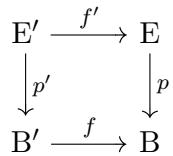
\includegraphics[keepaspectratio]{images/part001_eb35a58e.jpg}}

是一个笛卡尔方块。

事实上，映射 \(h: E' \to B' \times_{B} E\) （由 \(h(x') = (p'(x'), f'(x'))\) 定义的）是主纤维丛的 \(B'\)-态射，因而是同构；此外，我们有 \(pr_{2} \circ h = f'\)，由此得结果 (I, p. 8, prop. 2)。

在前一推论的假设下，有时称 \(f'\) 为主纤维丛的 f-态射。

命题 2. --- 设 (E, p) 为以 B 为基、以 G 为群的主纤维丛，设 \(\varepsilon\) 为截面 \(b \mapsto (b, e)\) （平凡主纤维丛 (B \(\times\) G, \(\mathrm{pr}_{1}\)) 的），其中 \(e\) 表示 G 的单位元。映射 \(h \mapsto h \circ \varepsilon\) 是从 \(\mathcal{C}_{\mathrm{B}}^{\mathrm{G}}(\mathrm{B} \times \mathrm{G}; \mathrm{E})\) 到连续截面所成之集 \(\mathcal{S}(\mathrm{B}; \mathrm{E})\) （\(p\) 的）上的双射。其逆双射把连续截面 \(s\) （\(p\) 的）对应到 B-态射 \((b, g) \mapsto s(b) \cdot g\)。

推论. --- 主纤维丛可平凡化，当且仅当它有连续截面。

命题 3. --- 设 E 与 B 为拓扑空间，\(p\colon\mathrm{E}\to\mathrm{B}\) 为连续映射，G 为右作用于 E 上的拓扑群。下列条件等价：

\begin{enumerate}
\def\labelenumi{(\roman{enumi})}
\item
  赋以映射 p 的 E 是以 B 为基、以 G 为群的主纤维丛；
\item
  对每个 \(x \in E\) 与每个 \(g \in G\) ，有 \(p(x \cdot g) = p(x)\) ，映射 \(\theta: (x, g) \mapsto (x, x \cdot g)\) 是 \(E \times G\) 到 \(E \times_{B} E\) 上的同胚，且 B 的每一点都有邻域，映射 p 在其上存在连续截面。
\end{enumerate}

(i)⇒(ii)：设 (E, p) 是主纤维丛。群 G 连续且自由地作用于 E，其轨道即 p 的纤维。于是映射 \(\theta\) 是双射且连续。更精确地说，若给 \(E \times_{B} E\) 赋以由 \((x, y) \cdot g = (x, y \cdot g)\) 定义的 G 的作用，则映射 \(\theta\) 是平凡主纤维丛 \(E \times G\) 到主纤维丛 \((E \times_{B} E \to E, \mathrm{pr}_{1})\) （例 5）中的 E-态射，因而是同构（命题 1）。(ii) 的其余断言由定义立即得出。

(ii)⇒(i)：令 \(\varphi = pr_{2} \circ \theta^{-1}\) ，于是对每个 \((x, y) \in E \times_{B} E\) ，有

\[
\theta^ {- 1} (x, y) = (x, \varphi (x, y)).\tag{1}
\]

映射 \(\varphi\colon\mathrm{E}\times_{\mathrm{B}}\mathrm{E}\to\mathrm{G}\) 是连续的，且对 \((x,y)\in\mathrm{E}\times_{\mathrm{B}}\mathrm{E}\)，元素 \(\varphi(x,y)\) 是 G 的唯一元素 \(g\) （使得 \(y=x\cdot g\) 的）。设 \(b\) 为 B 的一点；设 U 为 \(b\) 的邻域，\(s\) 为 \(p\) 在 U 上的连续截面。对 \((u,g)\in\mathrm{U}\times\mathrm{G}\)，令 \(f(u,g)=s(u)\cdot g\)；映射 \(f\) 是从 \(U \times G\) 到 \(\overline{p}^{-1}(\mathrm{U})\) 中的 U-态射。对 \(y\in\overline{p}^{-1}(\mathrm{U})\)，令 \(f'(y)=(p(y),\varphi(s(p(y)),y))\)。映射 \(f'\) 是从 \(\overline{p}^{-1}(\mathrm{U})\) 到 U \(\times\) G 中的 U-态射。我们有

\[
(f \circ f ^ {\prime}) (y) = s (p (y)) \cdot \varphi (s (p (y)), y) = y.
\]

另一方面，对 \((u,g)\in \mathrm{U}\times \mathrm{G}\) ，有

\[
(f ^ {\prime} \circ f) (u, g) = f ^ {\prime} (s (u) \cdot g) = (u, \varphi (s (u), s (u) \cdot g)) = (u, g).
\]

因此 f 是 U-同构。由此得出 \((E,p)\) 是以 B 为基、以 G 为群的主纤维丛。

注 1. --- 设 (E, p) 为以 B 为基、以 G 为群的主纤维丛。用命题 3 的记号，映射 \(\theta^{-1}\colon E \times_{B} E \to E \times G\) 是主纤维丛 \(\mathrm{pr}_{1}\colon E \times_{B} E \to E\) 的一个平凡化。称 \(\theta^{-1}\) 为这个主纤维丛的典范平凡化。

推论 1. --- 设 G 为连续右作用于拓扑空间 E 上的拓扑群。下列条件等价：

\begin{enumerate}
\def\labelenumi{(\roman{enumi})}
\item
  轨道空间 E/G 是 Hausdorff 的，且赋以典范映射 \(p: E \rightarrow E/G\) 的空间 E 是以 G 为群的主纤维丛；
\item
  群 G 逆紧地 (TG, III, p. 27) 且自由地作用于 E，且 E/G 的每一点都有邻域，映射 p 在其上存在连续截面。
\end{enumerate}

令 \(B=E/G\)。在假设 (i) 与 (ii) 的每一个之下，群 G 都连续且自由地作用于 E，于是映射 \(\theta\colon(x,g)\mapsto(x,x\cdot g)\) 是从 \(E\times G\) 到 \(E\times_{B}E\) 上的连续双射。我们置于这个假设之下，并用 \(\varphi\colon E\times_{B}E\to G\) 表示映射 \(pr_{2}\circ\theta^{-1}\)。顾及公式 (1)，\(\theta\) 是同胚，当且仅当映射 \(\varphi\) 是连续的。另一方面，由于 G 所定义的等价关系是开的 (TG, III, p. 10, lemma 2)，空间 E/G 是 Hausdorff 的，当且仅当这个等价关系的图 \(E\times_{B}E\) 在 \(E\times E\) 中是闭的。G 逆紧地作用于 E，当且仅当 \(E\times_{B}E\) 在 \(E\times E\) 中是闭的且映射 \(\varphi\) 是连续的。于是条件 (i) 与 (ii) 的等价性由命题 3 得出。

推论 2. --- 设 G 为拓扑群，H 为 G 的子群，p: G → G/H 为典范映射。若映射 p 在 G/H 的某个非空开集上有连续截面，则 p 使 G 成为以 G/H 为基、以 H 为群的主纤维丛。

通过左平移，G/H 的每一点都有邻域，映射 p 在其上有连续截面。另一方面，对 \((g,g')\) （属于 \(G\times G\) 的），令 \(\varphi(g,g')=g^{-1}g'\)。若 \(p(g)=p(g')\)，则 \(\varphi(g,g')\) 属于 H。映射 \((g,g')\mapsto(g,\varphi(g,g'))\) （从 \(G\times_{G/H}G\) 到 \(G\times H\) 的）是连续的，且是连续映射 \(\theta: G\times H\to G\times_{G/H}G\) （由 \(\theta(g,h)=(g,gh)\) 定义的）的逆，由此得该推论。

注 2. --- 这种情形特别出现于：G 是实李群，有限维、无穷可数，解析地且可迁地作用于解析流形 X。若取 H 为 X 的某点的稳定子，则映射 p 是 G 到齐性李空间 G/H 上的浸没，后者同构于 X (LIE, III, p. 109, corollary)。因此它有局部截面 (VAR, p. 50)。
% semantic-fragments: legacy-input-seam
\relax{}
